% newmicro (new_microarchitecture)
%
%\documentclass[10pt,dvips]{article}
%\documentclass[10pt,twocolumn]{article}
\documentclass[10pt,twocolumn]{IEEEtran}
%\documentclass[10pt]{IEEEtran}
\usepackage[english]{babel}
\usepackage{epsfig}
%\usepackage{fancyheadings}
%\usepackage[T1]{fontenc}
%\usepackage[latin1]{inputenc}
%\usepackage{twocolumn}
%\usepackage{verbatim,moreverb,doublespace}
%\usepackage{rotate,lscape,dcolumn,array,rotating,latexsym}
%
%\input{epsf}
%
% for somebody (I forget now !)
%\textwidth 175mm
%\textheight 225mm
%\topmargin -4.5mm
%
% for somebody else (I also forget now !)
%\textwidth 6.6in 
%\textheight 239mm
%\topmargin -15mm
%\leftmargin -2.0in
%
% for IEEE (single-column format)
\textwidth 6.875in
\textheight 8.875in
\topmargin -0.6in
%\oddsidemargin 0mm
%\evensidemargin 0mm
%
% for IEEE (two-column format)
\textwidth 6.5in
\textheight 8.875in
\topmargin -0.4in
%\oddsidemargin 0mm
%\evensidemargin 0mm
%
%
% some publishers want no page numbers for final print
\pagestyle{empty}
%
%
\begin{document}
%
% going to 1mm here recoups some good space ! :-)
%\parskip 1mm
\parskip 2mm
%
%
\title{A Ditributed Microarchitecture for Realizing High-ILP}
%
\author{
A. Khalafi, D. Morano, D.R. Kaeli\\
Northeastern University\\
{akhalafi, dmorano, kaeli}@ece.neu.edu\\
\and
A.K. Uht\\
University of Rhode Island\\ 
uht@ele.uri.edu
}
%
%
% some publishers do not want a data in the final print
%\date{}
%
%
\maketitle
%
% uncomment the following for page with no page numbers (for IEEE)
%\thispagestyle{empty}
%
%
\begin{abstract}
Many existing programs, and applications in general, are
very serial in nature and cannot easily be parallized
for gaining execution speed-ups.
Existing, conventional, microarchitectures have not
been able to extract large amounts of ILP from these sorts of
programs so far.
Rather, new, large, and more aggressive out-of-order microarchitectures
are needed for this task.
We introduce a new microarchitecture suitable for extracting
large amounts of instruction level parallelism (ILP) from sequential
oriented programs.
Instructions per clocks (IPC)
in the range of 3.8 to 5.1 are obtained for the
range of machine configurations studied running SpecInt-2000 and
SpecInt-95 programs. 
\end{abstract}
%
%
%\vspace{-0.25in}
\section{Introduction}
%\vspace{-0.15in}
%
\PARstart{W}{e} introduce a new distributed microarchitecture for achieving
a high amount of instructions per clock (IPC) from general 
sequential program codes.
Lam et al ~\cite{Lam92} showed that a large amount of instruction
level parallelism (ILP) is present within typical program codes.
Results by Uht et al ~\cite{Uht95} confirmed this and showed in more detail
how mimimal control dependencies and multipath execution are
important in exploting ILP.
Gozalez et al ~\cite{Gon97,gonzalez98limits }
also showed the potential for ILP when considering value prediction.
Suitable microarchitectures for extracting this ILP would need to
execute a very large number of instructions in parallel.
Unfortunately, conventional microarchitectures currently suffer
from hardware resource contention and routing congestion problems when
scaled to large sizes ~\cite{Palacharla97}.  
Particularly severe contention occurs for 
microarchitectures using
issue windows,
register update units, or reorder buffers~\cite{Smith95,Bannon95,Kessler98}.
Microarchitectures that have been proposed to attempt to mitigate
the problems associated with large numbers of parallel execution
resources have either relied, in part, on assistance from a
compiler, thus rendering them unsuitable for legacy instruction
set architectures (ISA).  
Microarchitectures such as the Multiscalar 
processor ~\cite{Sohi95} and the Grid Processor Architecture ~\cite{Nag01} 
have been of this type.  

Many microarchitectural ideas appear to offer potential for
exploiting ILP beyond what conventional designs can do.
Some of these ideas include multipath execution,
agressive control-flow speculation, value prediction, and
memory handling through aggressive memory disambiguation.
Some microarchitectures capable of mutlipath
execution include those described by Wang ~\cite{Wang90}, 
Uht and Sindagi ~\cite{Uht95},
Heil and Smith ~\cite{Heil96},
the PolyPath by Klauser et al ~\cite{Klauser98},
and a simultaneous multithreading oriented approach by
Wallace et al \cite{Wallace98}. 
Microarchitectures that aattempt to 
execute control-independent instructions
beyond the join of conditional branches (minimal control
dependencies) are described by 
Sankaranarayana and Skadron ~\cite{Sank01a,Sank01b}, 
Cher and Vijaykumar ~\cite{Cher01}, and Uht et al ~\cite{Uht01}.
Employing
value speculation ~\cite{ lipasti96exceeding,lipasti97performance }
also appears to be a significant advance in exploiting inherent ILP
by breaking the data dependence graph of the program.
A representative microarchitecture of this sort would
be the Superspeculative machine of 
Lipasti et al ~\cite{lipasti97superspeculative}.
Aggressive memory handling for large microarchitectures
was also proposed by Franklin et al ~\cite{Franklin96}.
And a promising mechanism for managing the problem of program
execution result ordering was employed in the 
Warp Engine ~\cite{Cleary95}.

Our goal was to attempt to combine the best features of
both existing microarchitectures and microarchitectural proposals,
along with new ways to handle problems associated with existing
designs.
We drew from many of the above ideas and propose a
space-distributed, scalable, grid-oriented microarchitecture
that features: multipath execution, minimal control
dependencies, value prediction, agressive memory speculation and
handling, and time tags for maintaining program dependency order.

The rest of this paper is organized
as follows.
Section 2  ...

Section 3 presents a description of 

Section 4  ...

We summarize in Section 5.
%


\section{Resource-Flow execution model}

One of our motivations for the design of a new microarchitecture was to
exploit as much speculation as possible.  We believe that achieving
high IPC requires going beyond the traditional data and control flow
dependency constraints in executing a program to allow for more
parallel execution of the code.  In current microarchitectures that
perform speculative execution, access to the reorder buffer becomes
very problematic as the number of instructions being speculatively
executed concurrently grows [D19].  This is mainly due to the
contention for the centralized resources such as data registers within
the reorder buffer.  In the proposed resource flow execution model the
instructions with the highest priority that are not yet executed are
assigned to free execution resources. The assignment is done regardless
of whether the input operands of the instructions have the correct
value (data flow constraints) and regardless of the outcome of the
branches (control flow constraints).  This means that the execution is guided
based upon the availability of resources.  The rest of the execution
time is spent re-executing the instructions that have had an incorrect
speculative input or operand, so as to end up with a programmatically
correct execution of the code.  As demonstrated in the rest of this
section, through application of the Resource-Flow execution model there
is no need for explicit renaming of registers or any reorder buffers
that would eliminate the contention for centralized resources.  This
model provides methods for executing standard control flow  programs
that go beyond the standard control flow model, the data flow model[U1]
and the Superspeculative model[U10].

\subsection{Time Tags}


In the Resource-Flow execution model, instructions are executed
speculatively in an out-of-order fashion.  We use time-tags to enforce
the correct data and control dependencies among the instructions to
realize speculative data-flow execution of code.  A time-tag is a small
integer that uniquely identifies the position of an instruction or an
operand in program ordered time with respect to the most recently
retired instructions.  %Time-tags are used in common processors to
squash instruction results occurring after a mispredicted branch, as
well as to maintain instruction order in general [].  Time-tags, as
used in our microarchitecture were originally proposed in the Warp
Engine [U2].  This machine relied on the use of floating point numbers
for the time-tags.  In our microarchitecture, time-tag values refer to
the issue slots in the execution window and are small integer values.

To assign the time-tags, the oldest issued instruction in flight that
is neither yet committed nor squashed would usually have a time-tag
value of zero.  More recently dispatched instructions take on
increasingly larger values the further ahead they are in the program
ordered instruction stream.  As a group of instructions with the lowest
value time-tags are retired, all of the time-tags for all instructions
and operands are decremented by the number of instructions just
retired.  This will keep the next instruction to be retired in having
the time-tag value of zero and therefore prevents time-tags from
growing indefinitely.

Both renaming and time-tagging assume \emph{forwarding} of instruction
result operands on a bus, snooped by all later instructions.  In the
resource flow model, the forwarding of the identifying address of the
output operand and its value is accompanied with the instruction
time-tag and path ID (if multipath execution is allowed) of the
forwarded result.  The time-tag and path ID will be used by subsequent
instructions in the execution window to determine if the operand has
the desired address value and therefore should be snarfed as an input
that will trigger its execution or re-execution.

\begin{figure}
%\vspace{0.2 in}
%\setlength{\epsfxsize}{10cm}%7
%\centerline{\epsfbox{window.eps}}
%\centering
\epsfig{file=source.eps,width=3.0in}
\caption{Operand snoop logic within an AS.}
\label{fig:source}
\end{figure}  
 
\begin{figure*}[th]
%\vspace{0.2 in}
%\setlength{\epsfxsize}{10cm}%7
%\centerline{\epsfbox{ttexec.eps}}
\centering
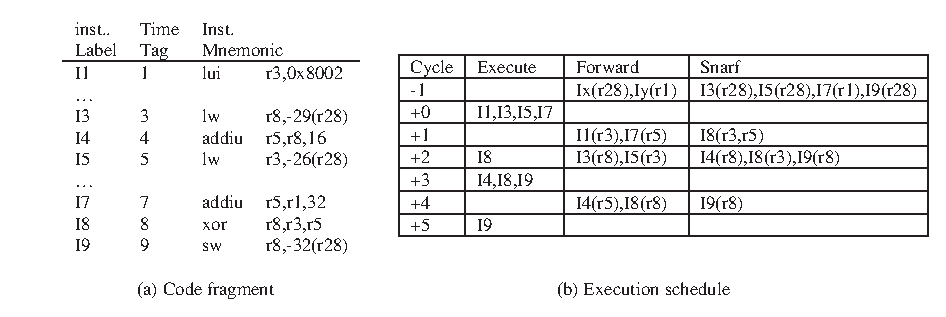
\epsfig{file=ttexec.eps,width=5.0in}
\caption{Example instruction exectuion.}
\label{fig:ttexample}
\end{figure*}  

The issue slots in our microarchitecture are modified to handle
instruction execution and forwarding and snooping of instruction
results.  We call this modified issue slot an Active Station (AS).
Figure~\ref{fig:source} shows the detailed snooping hardware for an
input operand of an Active Station. Basically, a new operand is snarfed
when it has the same address and path identifier(if multipath execution
is allowed) as the current AS, as well as a time-tag value that is less
than that of the current AS itself but greater or equal to that of the
last snarfed operand.

The information associated with each operand that is broadcasted from
one instruction to subsequent ones is referred to as a
\emph{transaction} , and generally consists of:

\begin{itemize}
\item Transaction type
\item Operand Type
\item Path ID
\item Time-tag of the originating instruction
\item Identifying address
\item Data value for this operand
\end{itemize}

True flow dependencies are enforced through continuous snooping of
theses transactions by each dispatched instruction residing in an
active station that receives the transaction.

Figure~\ref{fig:ttexample}  is an example of how time-tags are used to
enforce correct execution of instructions by enforcing data
dependencies.  Part (a) shows a fragment of a MIPS code.  For
simplicity, in this example we assume that there are no branches among
these instructions and at the end all of them will be committed.  Each
instruction is assigned to an active station with a unique time-tag.

Figure 2(b) illustrates the steps required to execute this code
fragment.  For simplicity, we assume that there is constraint on the
number of execution units and the number of transactions that can be
forwarded in each cycle.  The first column shows the relative clock
cycle times.  The next three columns list the instructions that are
either executing, forwarding an operand or snarfing a snooped operand
value.  The notation that is used is $I_x(r_y)$ where $I_x$ is the
instruction label and $r_y$ is the register that is either forwarded or
snarfed in.  Note that snarfing is done in parallel with instruction
execution or transaction forwarding.

At clock 0 instruction $I_1$, $I_3$, $I_5$ and $I_7$ are executed in
parallel.  The execution is the result of  snarfing of r1 and r28
registers in the previous cycle.  Assuming two cycles for the execution
of load and store instructions, and one cycle for the rest of the
instructions in this example, instruction $I_1$ and $I_7$ will produce
their results in the next clock.  The new value for register r3 and r5
is forwarded in clock 1 and is snarfed at $I_8$.   In the next clock,
instruction I8 will be executed using its newly-read register value.
Normally $I_8$ should forward the new result, but since I5 is sending
out a new value for r3, the $I_8$ instruction snarfs the new value of
r3. This results in re-execution of $I_8$ instruction at clock +3.  In
the next cycle, $I_4$ sends a new value for register r5 with a time-tag
of 4, but since the last value of $r5$ received by $I_8$ had a time-tag
of 7, which is greater than 4, the new value is ignored by $I_8$ and
does not result in another re-execution.

\subsection {Memory operations}

With the increasing number of instruction in flight, there is a higher
probability that the memory values generated by store operations will
be used by other load operations in the exectuon window.  Tabel xx
shows the ratio of memory operations that can get their operand values
directly from other instruction in the execution window withot having
to go to a higher level of memory hierarchy.  This means that if we
could somehow satisfy a portion of the memory operations in the
execution window, it would result in less pressure on the higher levels
of memory hierarchy and overall performance improvement.

To enforce the true memory dependencies, we could still use the
forwarding and snooping mechanism introduced in the last section.
There are, however, limitations to the applicability of this approach.
Unlike with register operands, the architected address for a memory
operand is not fixed.  The memory address is generally computed using a
fixed displacement and a register value.  Due to the speculative nature
of this microarchitecture, the register value for the memory operation
could be incorrect, resulting in a wrong memory address.

A load operation that snoops for an incorrect memory address will miss
the opportunity to snarf the correct memory value forwarded by a
previous store operation.  It is therefore necessary for a load
operation to initiate a memory request using its resolved memory
address.  In traditional microarchitectures, the request normally goes
to the first level D-cache.  In our proposed microarchitecture, there
is a good chance that the memory value is still in the execution window
and has not yet written back to the higher level memory.  Based on this
observation, we need to send the memory requests to both higher level
memory and previous active stations.  If there is any store operation
with the same address in the earlier active stations, it will forward
the memory value, which subsequently, will be used by the load
instruction.  Otherwise the memory value received form the higher level
memory is used.  The requests to the higher level memory, are sent
using a set of shared horizontal buses.  The requests to the previous
active stations are handled using a set of backwarding buses. These
buses are essentially similar to the forwarding buses except that they
are primarily used to send data requests to the instructions earlier in
the program order.   More discussion on memory structure and busing
will be presented in later sections.

Another difficulty with the application of the forwarding and snooping
strategy for memory operations is that a store operation with an
incorrect memory address could forward an erroneous value that will be
incorrectly snarfed by another load operation with the same address.
This presents a problem for the correct enforcement of memory operand
dependencies.  We solved this by forcing the store operation to notify
subsequent load instructions to ignore its previously forwarded value.
We define \emph{nullify} transaction as a new type of transaction with
the property of canceling the effect of a previous store transaction.
Any store instruction that has previously forwarded a memory value with
the incorrect speculative address, will send a nullify transaction upon
re-execution.  This transaction is seen by all later load
instructions.  Any load instruction that has snarfed a value sent from
that specific store instruction will ignore the value and sends a new
request to the memory and on the backwarding buses.

\subsection {Hardware Predication}

Predicated execution is shown to be an effective approach for handling
conditional branches [].  In our microarchitecture, the predicates are
generated at run-time.  Each instruction computes its own enabling
predicate by snooping for and snarfing predicate operands that are
forwarded to it by earlier instructions from the program-ordered past.
They are evaluated solely with hardware, allowing the use of legacy
code.  Full hardware based predication is a new way to manage and
achieve Minimal Control Dependence.  With MCD, all branches may execute
concurrently, and the instructions after a branch domain [U15] may
execute independently of the branch.

\begin{figure}
%\vspace{0.2 in}
%\setlength{\epsfxsize}{10cm}%7
%\centerline{\epsfbox{window.eps}}
%\centering
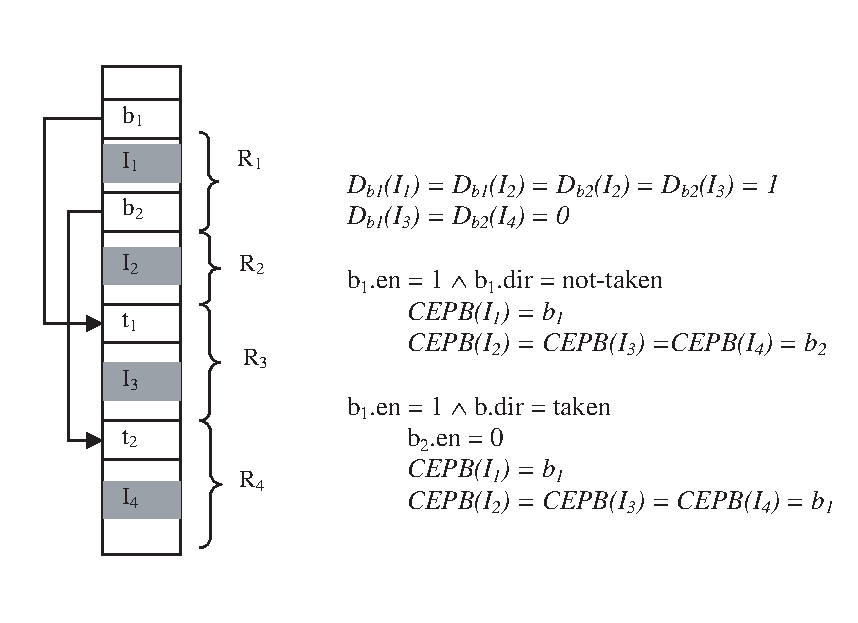
\epsfig{file=brdomain.eps,width=3.0in}
\caption{Branch Domains and Closest Enabled Previous (CEP) Branch.}
\label{fig:brdomain}
\end{figure}  
 
In this section we propose a hardware predication mechanism that can be
implemented using our resource flow methodology.
Figure~\ref{fig:brdomain} shows a program code sequence with two
branches $b_1$ and $b_2$.  with corresponding targets $t_1$ and $t_2$.
The two branches divide the code into 4 regions.  The execution of the
instructions in regions $R_1$, $R_2$ and $R_3$ depends on the outcome
of the $b_1$ and $b_2$ whereas the instructions in $R_4$ are executed
independent of the branch outcomes.  In this section, we are proposing
a new scheme for assigning an enabling predicate to every instruction
in each region based on the outcome of branches.  If the enabling
predicate value is one, then the instruction will be executed;
otherwise it is disabled.  The following definitions are used in the
description of our scheme.

\vspace{0.2 in}
\begin{description}[\setlabelwidth{CEP(Ij)xxx}]
\item[$T_b$:] a binary value, set to one if the branch $b$ is predicted 
taken
\item[$ex_j$:] a binary value assigned to each instruction $I_j$ and 
specifies whether the instruction is executed or otherwise disabled.
\item[$D_b(I_j)$:] a binary value, set to one if the 
instructions $j$ is in the 
domain of branch $b$.
\item[$CEP(I_j)$:] Closest Enabled Previous branch to instruction $I_j$ in 
the static program-order.
\end{description}
\vspace{0.2 in}

\begin{figure}
%\vspace{0.2 in}
%\setlength{\epsfxsize}{10cm}%7
%\centerline{\epsfbox{window.eps}}
%\centering
\epsfig{file=dynpred.eps,width=3.0in}
\caption{Example of how Dynamic Predicate works.}
\label{fig:dynpred}
\end{figure}  

Figure~\ref{fig:brdomain}i(b) shows an example along with the value of
some the variables defined above.  The $D_b(I)$ function is independent
of the outcome of the branch as only depends on the static order of
instructions in the code.  $CEP(I)$, on the other hand, is a function
of the outcome of other branches and will change during the course of
speculative execution.

Using the above definitions, we can see that

$\overline{ex_j} = T_b \cdot D_b(I_j)$  where $b = CEP(I_j)$.   (1)

This equation simply tells us that if an instruction $I_j$ is in the
domain of an enabled branch, and the branch is taken, it will not be
executed.  If the branch is out of the domain, then its execution is
independent of the outcome of the branch.

Equation (1) is the base for our dynamic predication scheme.  To set
the predication for each instruction $I_j$, it is sufficient to find
the $CEP(I_j)$ branch and its outcome.  This is a simple task in our
scheme.  Each active station has a pair of $CEP\_TT$ registers to keep
the time-tag of its current $CEP$ branch and corresponding target.  If
an earlier branch is enabled, a \emph{Predicate} transaction is sent on
the forwarding bus with the branch time-tag, its target address and
whether it is a taken branch or not. Each subsequent instruction that
snoops this transaction checks to see if the time-tag of the newly
enabled branch is greater than its current $CEP\_TT$ value. If so, the
new branch is closer to this instruction and therefore it will replace
the older $CEP$ branch.

If a branch such as $b$ is disabled, the later instructions need to
obtain the new $CEP$ branch.  The new branch is simply $CEP(b)$ because
there is no other enabled branch between it and $b$.  In our scheme
this is handled by forwarding an invalidate transaction by branch $b$.
An invalidate transaction contains the time-tag of $b$, the time-tag of
$CEP(b)$ and the branch domain information of $CEP(b)$.  This
information was stored at $b$ when $CEP(b)$ forwarded its predicate
transaction.

To find the domain of a $CEP$ branch, a simple approach is to just
compare the branch target address with the instruction address.  It is
a however better to use time-tags for this purpose.  To do so, a branch
needs to forward the time-tag of its target instruction instead of its
target address. The branch target time-tag can be easily calculated by
adding the branch displacement to the branch time-tag value.

Another improvement to the above scheme can be made by noticing that a
not-taken enabled branch does not need to send out any transaction on
the forwarding bus.  This is due to the fact that a not taken branch
essentially acts like a NOP operation.  The advantage is a reduction of
the number of transactions on the bus.  Figure~\ref{fig:dynpred} shows
an example of how our dynamic predicate work.  The first column in the
table lists the relative clock cycles.  The next three columns list the
status of each branch.  The "D", "T' and "NT" entries correspond to
disabled, taken and not-taken status respectively.  The next two
columns list the $I_k$ Instruction status.  "E" and "D" stand for
enabled and disabled status respectively.  The $CEP$ column shows the
$CEP(I_k)$ branch at any cycle.  The next two columns show the
transactions on the bus.  The "pred." column lists the predicate
forward transactions for each branch along with its status.  The
"inval." column lists the invalidating transactions.  the branch name
in the parenthesis corresponds to the new CEP forwarded by the
invalidated branch.

In the example, it is assumed that $b_1$ and $b_3$ are initially
predicted taken and not-taken respectively and a as a result $I_k$ is
enabled.  In the next clock, $b_1$ changes its direction to a not-taken
branch and sends a forwarding transaction on the bus.  This transaction
will enable $b_2$ which is also predicted taken.  $b_2$ will send a
predication transaction on the forwarding bus which is snooped by
$b_3$.  As a result, $b_3$ will be disabled in clock 3 and will send an
invalidating transaction with $b_2$ as its $CEP$ branch.  instruction
$I_k$ will see this transaction and switch its $CEP$ to $b_2$ and as a
results will be disabled.  The bottom section of the table in figure xx
shows what will happen if $b_1$ changes back to a taken status.  A new
set of transactions will follow that eventually enable $I_k$.

In the previous example we saw that $I_k$ was first disabled and then
enabled.  A disabled instruction needs to notify \emph{later}
instructions that its destination register value, which could have been
forwarded earlier, is not valid anymore.  Further, it has to send the
old destination value from the closest enabled previous instruction as
the correct value.  This is done through a relay transaction where the
previous value is sent out as the new value produced by this
instruction.  The disabled instruction, in effect acts like a relay and
will forward the earlier value using its own time-tag.

As demonstrated by this example, the cost of hardware predication is
low, since most of the extra state storage only takes a few bits in the
AS.  This hardware stays same for all active stations and columns

\section {A Resource Flow Microarchitecture}

In this section we present an ISA independent, scalable, distributed
microarchitecture that uses Resource Flow execution model and some of
the most desirable features of future microarchitectures in order to
achieve large IPC.  Among these are control flow speculation,
control-independent and multipath execution.  The microarchitecture is
very aggressive in terms of the amount of speculative execution it
performs.  This is realized through a large amount of scalable
execution resources.  Resource scalability of the microarchitecture is
achieved through its distributed nature along with repeater-like
components that limit the maximum bus spans.  Contention for major
centralized structures such as register file, reorder buffer and
centralized execution units are eliminated through distribution of
theses resources.

\begin{figure}
%\vspace{0.2 in}
%\setlength{\epsfxsize}{10cm}%7
%\centerline{\epsfbox{window.eps}}
%\centering
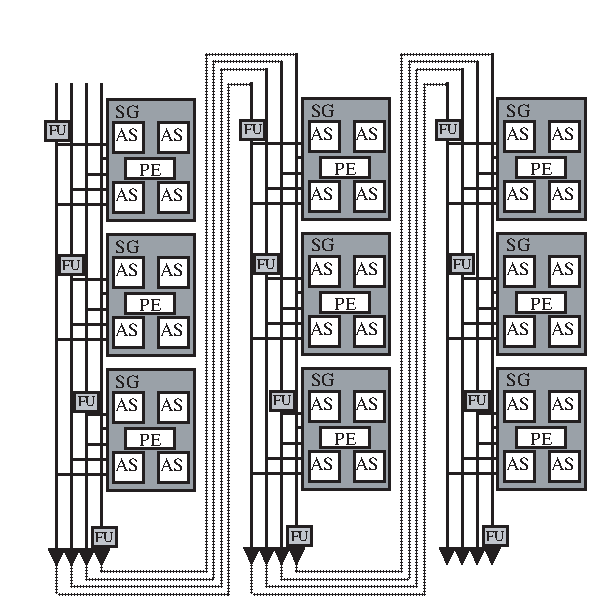
\epsfig{file=execwind.eps,width=3.0in}
\caption{Interconnection fabric in the Execution Window.}
\label{fig:execwind}
\end{figure}  

Figure~\ref{fig:execwind} shows a partial diagram of our execution
window with its subcomponents.  The active stations are laid out in a
two dimensional grid where sequentially loaded instructions go to
sequential active stations down a column.  The use of a two dimension
grid simply provides a means to implement the necessary hardware in a
chip.

%The number of active stations in the height dimension of the grid is
%defined to be the column height.

Dispersed among the active stations are associated execution units.  An
execution unit is represented in the figure as processing element
(PE).  Processing elements may consist of a unified all-purpose
execution unit capable of executing any of the possible machine
instructions or, more likely, consist of several functionally
partitioned units individually tailored for specific classes of
instructions (integer ALU, FP or other), as is typical of most current
machines.  Groups of active stations along with their associated
processing elements are termed a sharing group (SG).

Sharing groups have a relatively high degree of bus interconnectivity
within them, as conventional microarchitectures do. The Active stations
serve the role of both the reservation station and the reorder buffer
of more conventional machines. The transfer of a decoded instruction,
along with its associated operands, from an AS to its PE is isolated to
within the given SG. The use of this execution resource sharing
arrangement also allows for reduced interconnections between adjacent
sharing groups. Basically, only operand results need to flow from one
SG to subsequent ones.

\subsection {Segmented Buses}

An interconnection fabric is provided to forward result operands from
earlier active stations to later active stations in program order.  The
interconnect allows for arbitrary numbers of sharing groups to be used
in a machine while still keeping all bus spans to a constant length.
All the buses in Figure~\ref{fig:execwind} form the interconnection
fabric.  The width of the buses can be increased by using several buses
in parallel which will increase the overall bus bandwidth.

Active bus repeater components are required to allow for constant
length bus spans.  Adjacent bus segments are connected via Filter Units
(FU).  These units do more than just repeat operand values from one
span of a bus to the next.  For registers and  memory, operands are
filtered so that redundant forwards of the same value are eliminated.
This filtering provides a means to reduce the overall bandwidth
requirements of the forwarding interconnection fabric.  There are three
kinds of filter units.  The Register Filter Unit (RFU), Memory Filter
Unit (MFU) and Predicate Filter Unit (PFU).  Each type handles its
corresponding transactions.  Each RFU holds the most recent value with
the highest time-tag for each of the architected registers.  The
register values are then forwarded to the next bus segment during the
course of execution.
The MFU has basically the same structure of an RFU but it uses a small
cache (L0 cache) to store the latest forwarded memory values.  L0
cache proves to be an effective device in reducing the number of
requests to L1 D-cache.  However the limited size of L0 cache requires
periodic writes to the L1-D cache.  Among our filtering units, the PFU
are the simplest ones.  All they need to do is to keep track of the
latest CEP branch and forward it to the next bus span.

Register filter units result in the elimination of a centralized
register file and simplification of state commitment.  By the time that
the instructions in a column have gone through their final execution
and the column is ready to commit, the RFU's in this column have
already forwarded the register values to the RFU's in the later
columns.  Therefore it is unnecessary to save the ISA register state in
a separate register file.

As can be seen in figure~\ref{fig:execwind}, the buses go from the
bottom of each column to the top of the next column.  The bottom of the
last column in the execution window is connected to the top of the
first column.  This will create a loop where there is not really a
first or last column but there are \emph{earliest loaded column} (ELC)
and the \emph{latest loaded column} (LLC).  The operand values are
forwarded from each column to the next column, except for the LLC
column which will forward its operand values only when the ELC column
is committed and loaded with a new set of instructions.

\subsection {Multipath Execution}

Control-flow misprediction penalties pose an obstacle for designing
high performance microarchitectures.  Both MCD and Disjoint Eager
Execution (DEE) techniques are needed for achieving very high ILP
[U16].  DEE gives the highest priority for the use of execution
resources to the instructions with the highest likelihood of being
committed.  In our microarchitecture, the likelihood is not explicitly
calculated; instead the \emph{"static tree"} heuristic of [U16] is
used.  This is a form of multipath execution in which there is a
predicted or mainline path as well as several much shorter
not-predicted or \emph{disjoint} paths spawning from the mainline path
at some conditional branches.

DEE paths are created by loading a free second column of active
stations within a SG column.  Instructions from both mainline and
disjoint paths share the same PE and bussing resources in each sharing
group.  Active stations on the Mainline path, however, always have
priority for the use of resources.  In our present microarchitecture,
we always have two columns of active stations within a SG. The first AS
column is reserved for the main-line path of the program. The second
column of Active stations is reserved for the possible execution of a
disjoint path.  The cost impact of realizing DEE is however relatively
low and is usually less than 10 percent increase for a 45 precnet
performance improvement.

Mainline and disjoint paths execute concurrently, greatly reducing
branch misprediction penalties.  Conditional branches are assigned to a
free disjoint path (the path is \emph{spawned}) after they enter the
execution window.  The column with the disjoint path could be any free
column in the execution window and not necessarily the same column as
their mainline path column. This allows for multiple disjoint paths for
a single mainline path.  At branch resolution,  if the disjoint path
turns out to be the correct path, it will replace the mainline path and
the execution will continue form there. A detailed description of DEE
can be found in [].

\subsection {Instruction Fetch}

\begin{figure}
%\vspace{0.2 in}
%\setlength{\epsfxsize}{10cm}%7
%\centerline{\epsfbox{window.eps}}
%\centering
\epsfig{file=highlevel.eps,width=3.0in}
\caption{High level diagram of our microarchitercture.}
\label{fig:highlevel}
\end{figure}  
 
The challenge in high bandwidth instruction fetch is mainly concerned
with the problem of multiple-branch prediction and aligning and
collapsing of multiple fetch groups.  One approach for solving this
problem has been focused on enhancing the instruction cache by using
multi-ported, multi banked copies of the instruction cache[][][].  A
more recent approach has been the use of trace caches[][].

A high level diagram of our microarchitecture is shown in
figure~\ref{fig:highlevel}.  We are using a set of replicated
multiported I-caches to satisfy our high fetch bandwidth requirements.
Instruction are loaded in the active stations using a set of horizontal
buses  The key here is that instructions with small branch domain size
are normally fetched in the static or memory order.  This will simplify
the aligning and collapsing logic in the I-fetch unit.

Instructions are fetched by the I-fetch unit using a multiple branch
predictor [] and the following heuristics:

If a conditional backward branch is predicted taken, the I-fetch unit
will follow the taken path and continue loading instructions into the
execution window for the mainline path from the target of the branch.
A disjoint path is also spawned to speculatively execute the
instructions after the branch.  This heuristic allows for the capture
of program loops within the execution window of the machine.

In the case of forward branches, we define two threshold values,
\emph{Near Threshold} and \emph{Far Threshold}.  We then compare the
branch domain size with this threshold values which will categorize a
branch as one of \emph{near}, \emph{midway} or \emph{far}.

Since the domain of a forward near branch is small and can be easily
loaded within the execution window, the fetch unit will load the
instruction following the not-taken path of the branch, whether or not
it is the predicted path.  This represents fetching of instructions in
the memory or static order rather than the program dynamic order and is
very common in the absence of a loop.  The fetching and loading of
instructions following the not-taken output path of a conditional
branch is very advantageous for capturing hammock styled branch
constructs.  Simple single-sided hammock branches are generally have
near targets and are captured within the execution window.  These
branches are also good candidates for spawning a disjoint path which
can further reduce the misprediction penalties.

If the branch is a midway branch, then based on its prediction
confidence, the instructions are fetched from either the target of the
branch or subsequence instructions after the branch based on the
outcome of the branch predictor.

In the case of a far branch, we will always follow the predicted path
altough if the branch is predicted not taken, there is an apportunity
for spawning a disjoint path.
The threshold values are parameters that can be either fixed at 
design time or adaptively changed during the course of execution. 

\subsection {Execution Control}

In the last section we discussed as how I-fetch unit  fetches
instructions from I-cache along one or more predicted paths.
Instructions are then decoded and staged into an instruction load
buffer so that they are available to be loaded into the execution
window.  adjacent columns are loaded subsequently until the whole
window is full.  After that every time a column is committed and the
its instructions are retired, a new set of instructions are loaded into
that column.  Branch mispredictions can have different effects on the
execution.  speculative mispredictions of branches that their domain is
in the window results in a change of predicates and is handled through
resource flow execution.  If the branch has a disjoint path and
resolved to be mispredicted, a switch to the disjoint path is made.
The last case is when the branch is resolved to be mispredicted and the
instructions after the branch target had been fetched into the window.
In this case the execution window has to be \emph{flushed} and fetch
will resume after the branch.

A column can be committed when all the instructions in the column have
been executed and there are no more transactions on any buses
interconnecting the sharing groups in the column.  As we mentioned
before, there is no need for a centralized register file in this
architecture.  The L1-D cache, however, needs to be updated with the
store values not yet written back to it.  The previous column buffers
(PCB) in figure~ref{fig:hgihlevel} are used  for this purpose.  The PCB
snoops the bus looking for the stores from the previous column and
holds only the latest value for a given memory store address.  PCB is
used to distribute the store buffering throughout the machine and
reduce the amount of buffered information.

\subsection {Memory System}

Throughout the paper, we introduced some of the features of this
microprocessor that affect the memory system, including Memory Filter
Units, L0 cache, PCB and memory operations in the context of
resource-flow execution.  The above features are mainly effective
inside the execution window.  A set of replicated copies of multiported
non-blocking L1 D-cache are used to provide us with the necessary
bandwidth and low miss rate.  We also used a unified L2 cache

\section {Evaluation}

Baseline, IPC v.s. Geometry, Sensitivity data (Forwarding Units, Bus
Span, Memory and L1), Effect of DEE, effect of MFU and L0 cache,
execution window statistics, effent of changing the threshold values on
the I-fetch performance.

Many machine sizes have been explored so far but only a subset of these
sizes is further investigated in this paper. A particular machine is
generally characterized using the tuple:

\begin{itemize}
\item sharing group rows
\item active station rows per sharing group
\item sharing group columns
\end{itemize}

These three characteristic parameters of a given machine are greatly
influential to its performance, as expected, and is termed the geometry
of the machine. These three numbers are usually concatenated.  For
example the geometry of the machine in Figure~\ref{fig:highlevel}
 would be abbreviated 3-4-2.

\bibliographystyle{latex8}
\bibliography{newmicro}

%\begin{thebibliography}{11}
% Note the sample label "11" in thebibliography
% This is like the new IEEEtran class'
% \begin{enumerate}[\setlabelwidth{11}]
%\bibitem{something}
%{\em The Entries go here!!}
%
%\end{thebibliography}
%\vspace{1ex}\hrule\vspace{3ex}

\end{document}
